
%\setcounter{chapter}{8}
%\noindent
%\begin{Large}
%{\bf Lecture 8 \newline
%Compatibility of Observable: version 2}
%\end{Large}

\section{Background Materials}
Suppose that $\hat{A}$ is the Hermitian operator representing an observable A of a quantum system. The eigenkets of ${\hat A}$
form a complete set of orthonormal basis states. Let $|\psi\rangle$ be the state vector of the system. We can expand 
$|\psi\rangle$ in the eigenbasis of the operator ${\hat A}$:
\be
|\psi\rangle = \sum_a |a\rangle \langle a|\psi\rangle \, , 
\label{aeq:1}
\ee
where $a$ runs over all the eigenvalues of ${\hat A}$, i.e., $a\in {\rm spec}(\hat{A})$, where ${\rm spec}\,(\hat{A}) =
(a_1,a_2, a_3, \ldots )$ is the set of all eigenvalues of $\hat{A}$. This set is called the eigenvalue spectrum of $\hat{A}$.


\paragraph{}
In Eq. (\ref{aeq:1}), we have assumed that each eigenvalue $a$ is non-degenerate, i.e., for each $a$ there exists only one linearly independent eigenvector $|a\rangle$. Therefore, the eigenvalue itself can be used to label the corresponding eigenket unambiguously.

\paragraph{}
However, it may so happen that some or all of the eigenvalues of ${\hat A}$ are degenerate, i.e., there may be more than one linearly independent eigenvector corresponding to the same eigenvalue. The number of linearly independent eigenvectors corresponding
to a particular eigenvalue $a$ is called the order of degeneracy of the eigenvalue and is denoted by $g_a$. If the eigenvalue $a$ is degenerate, then just the eigenvalue itself is not enough to label the eigenstates uniquely. We need another index to distinguish between the $g_a$ linearly independent eigenvectors all with the same eigenvalue $a$.

\paragraph{}
Thus the eigenvectors belonging to a degenerate eigenvalue $a$ may be denoted by $|a,i\rangle$, where the index $i$ 
can take discrete values $i=1,2,3, \cdots , g_a$. The index $i$ may be called the degeneracy index. Later, we will see that we can improve the notation by replacing $i$ by the eigenvalues of other Hermitian operators $\hat{B}$, $\hat{C},\, \cdots$, which commute
with $\hat{A}$. 

\paragraph{}
The set of linearly independent eigenvectors $\{ |a,i\rangle, i=1,2, \cdots, g_a\}$, all with the same eigenvalue $a$, span a $g_a$-dimensional subspace of the Hilbert space. This subspace is called the eigensubspace of $a$, and is denoted by $H_a$. The union of all the eigensubspaces of the operator $\hat{A}$ constitutes the full Hilbert space.

\paragraph{}
It is easy to see that any linear combination of the eigenvectors $\{ |a,i\rangle, i=1,2, \cdots, g_a\}$ is also an eigenvector of $\hat{A}$ with the same eigenvalue $a$. Thus
\be
\hat{A} \left( \sum_{i=1}^{g_a} c_i |a,i\rangle\right) = a \left(\sum_{i=1}^{g_a} c_i |a,i\rangle\right)\,,
\ee
where $c_i$'s are constants.
The set of eigenvectors $\{ |a,i\rangle, i=1,2, \cdots, g_a\}$, even though linearly independent, may not be orthogonal to each other
because they belong to the same eigenvalue. However, following the Schmidt orthonormalization procedure, we can take linear combinations of the above set of vectors in a special way and obtain a set of $g_a$ orthonormal vectors. The new set of orthonormal (and hence also linearly independent ) vectors remain eigenvectors of $\hat{A}$ with the same eigenvalue $a$. 

\paragraph{}
We assume that the Schmidt procedure has been carried out in each eigensubspace. So, in each eigensubspace, we can write
\be 
\langle a,i|a,j\rangle = \delta_{ij} , \;\; a\in {\rm Spec}(\hat{A})
\ee
where $i,j = 1,2,3, \cdots , g_a$. 
The orthonormal set of eigenvectors $\{ |a,i\rangle, i= 1,2, \cdots , g_a\}$ can be said to span the eigensubspace $H_a$.
The eigenvectors in different eigensubspaces are automatically orthogonal because $\hat{A}$ is Hermitian. Hence, we can assume that 
{\bf all}  eigenvectors of $\hat{A}$ are orthonormal, i.e.,
\be
\langle a^{\prime}, i^{\prime}|a,i \rangle = \delta_{aa^{\prime}}\delta_{ii^{\prime}} \, .
\ee
The full set $\{ |a, i\rangle, i=1,2, \cdots , g_a;\, a\in {\rm spec}\,(\hat{A}) \}$ of eigenvectors of $\hat{A}$ form a complete 
orthonormal set, i.e., they constitute a basis set for the Hilbert space. The completeness condition of this basis set can be written as 
\be 
\sum_{a\in {\rm spec}\,(\hat{A})}\sum_{i=1}^{g_a} |a,i \rangle \langle a,i| = \hat{I}\, .
\ee
Thus the state vector $|\psi\rangle$ of the system can be expanded as
\begin{eqnarray}
|\psi\rangle & = & \hat{I} |\psi\rangle \nonumber \\
             & = & \sum_{a\in {\rm spec}\,(\hat{A})}\sum_{i=1}^{g_a} |a,i \rangle \langle a,i|\psi\rangle\, .
\end{eqnarray}			

\paragraph{}
For simplicity, we will continue to use Eq. (\ref{aeq:1}) as the expansion for $|\psi\rangle$ in the eigenbasis of $\hat{A}$
assuming that all the eigenvalues are non-degenerate. In case of degeneracy, notations can be generalized in a straightforward manner, as discussed above.			



% Section 2
\section{Measurement of Two Observables in Quick Succession}
Suppose that a quantum system is in the state $|\psi\rangle$. Let $A$ be an observable of the system with corresponding Hermitian operator $\hat{A}$. We can always expand $|\psi\rangle$ using the eigenbasis of $\hat{A}$:
\be
|\psi\rangle = \sum_a |a\rangle \langle a|\psi\rangle \, ,
\ee
where $a$ runs over the eigenvalue spectrum of $\hat{A}$. The complex number $\langle a |\psi\rangle$ is the `component' of 
$|\psi\rangle$ along $|a\rangle$. 

\paragraph{}
We now make a measurement of the observable $A$ on the system in the state $|\psi\rangle$. Since a general state $|\psi\rangle$
may be a superposition of many (perhaps infinitely many) eigenkets of $\hat{A}$ with different eigenvalues, we cannot exactly 
predict the result of the experiment but can only say that the experiment would yield one of the eigenvalues 
of $\hat{A}$ for which $\langle a|\psi\rangle \neq 0$. 

\paragraph{}
The outcome is random, i.e., probabilistic, because we cannot predict exactly which eigenvalue will be obtained, but we can assign a probability for obtaining a particular eigenvalue $a$ provided we know the state $|\psi\rangle$ before the measurement.
The probability is
\be
P_{|\psi\rangle}(a) = \left|\langle a|\psi\rangle \right|^2 \, . 
\ee
In the course of the measurement, the state of the system collapses to the eigenket $|a\rangle$ if the eigenvalue $a$ is obtained in the measurement. Thus
\be
|\psi\rangle\;\; \xrightarrow{{\rm measurement\; of\; A} }\;\; |a\rangle.
\ee
Now the system is in a state with a definite value for the observable $A$. Further successive measurements of $A$ will yield the same eigenvalue $a$ with 100\% certainty. 

\paragraph{}
Next, consider another observable $B$ of the system with corresponding Hermitian operator $\hat{B}$. If, immediately after the  measurement of $A$, we measure B, are we certain to get a particular eigenvalue $b$ of the operator $\hat{B}$?
We know that the state of the system after the measurement of $A$ is an eigenstate of $\hat{A}$, i.e., in a state with a definite value $a$ of the observable $A$. The question we have asked can be restated as follows: in the collapsed state
$|a\rangle$, does $B$ have a definite value, i.e., is $|a\rangle$ also an eigenstate of $\hat{B}$  with some eigenvalue $b$? The answer to this question is, in general, in the negative, i.e., $|a\rangle$ is not an eigenket of $\hat{B}$ in general. The very important exceptional case 
where $|a\rangle$ is also an eigenstate of $\hat{B}$ is discussed later.

\paragraph{}
Since the eigenkets of $\hat{B}$  form a basis set, we can expand $|a\rangle$ as
\be
|a\rangle = \sum_b |b\rangle \langle b|a\rangle \, .
\ee
Therefore, a measurement of $B$ would yield any one of the eigenvalues $b\in {\rm spec}\,(\hat{B})$ for which $\langle b |a\rangle \neq 0$.
The probability of obtaining a particular eigenvalue $b$ while the system is in the state $|a\rangle$ is
\be
P_{|a\rangle}(b) = \left | \langle b | a\rangle \right|^2 \, .
\ee
The state of the system after B is measured collapses from $|a\rangle$ to $|b\rangle$:
\be
|a\rangle\;\; \xrightarrow{{\rm measurement\; of\; B} }\;\; |b\rangle.
\ee
Thus, the measurement of $B$ generally alters the state of the system just before the measurement because, due to the measurement process, the system is thrown into the eigenstate $|b\rangle$, where $b$ is the eigenvalue of  $\hat{B}$ obtained in the measurement. But, since $|b\rangle$ is not, in general, an eigenstate of $\hat{A}$, the system is no longer in a state with a definite value for the observable  $A$.

\paragraph{}
If we measure $A$ again immediately after $B$ is measured, we will not get the answer we got the first time, namely $a$, with certainty. In the second measurement of $A$ there is the possibility of getting any eigenvalue for which $\left| \langle a|b\rangle\right| \neq 0$. To repeat,  after the first measurement of $A$, the system is in the eigenstate $|a\rangle$ of
$\hat{A}$ but this state is not an eigenstate of the operator $\hat{B}$ except in a special situation discussed below. After the measurement of $B$, the system is thrown in the eigenstate $|b\rangle$ of $\hat{B}$ which is not an eigenstate of $\hat{A}$. Therefore, it is not possible, in general, to get the system in a state in which both the observables $A$ and $B$  have definite values.

\paragraph{}
Now, in successive measurements of $A$ and $B$, first $A$ then $B$, on a system initially in the state $|\psi\rangle$, the probability of obtaining the result $a$ and $b$ is
\be
P(a,b) = P_{|\psi\rangle}(a) P_{|a\rangle}(b) = \left|\langle a|\psi\rangle\right|^2\left| \langle b|a\rangle\right|^2\, .
\ee
If we reversed the order of measurements, first $B$ and then $A$,  the probability for obtaining the results
$b$ for the observable $B$ and $a$ for the observable $A$ would be
\be
P(b,a) = P_{|\psi\rangle}(b) P_{|b\rangle}(a) = \left|\langle b|\psi\rangle\right|^2\left| \langle a|b\rangle\right|^2\, .
\ee
We note that, since $\left|\langle a|\psi\rangle\right|^2\neq \left|\langle b|\psi\rangle\right|^2$, the two probabilities are not equal in general, 
i.e., $P(a,b)\neq P(b,a)$.


% New Section

\section{Compatible Observables}
Now, let us return to the exceptional situation mentioned in the previous section. To recapitulate, let us make two 
measurements of two observables $A$ and $B$ in quick succession on a system in the state $|\psi\rangle$. First, we measure $A$, and if the eigenvalue $a$ is obtained, the system's state collapses to an eigenstate of the operator $\hat{A}$ belonging to the eigenvalue $a$. Then if we measure $B$ immediately afterward, would we be certain to get a particular eigenvalue $b$ of $\hat{B}$? Further, if a second measurement of $A$ is made immediately after the measurement of $B$, what conditions need be fulfilled in order that the result of the first measurement is unaltered, i.e., we will be certain to get the same result $a$ again? We will first consider the case when all eigenvalues of $\hat{A}$  and 
$\hat{B}$ are non-degenerate and then we will consider degeneracy of the eigenvalues. 

\subsection {Nondegenerate Case}
Suppose all eigenvalues of $\hat{A}$ and $\hat{B}$ are nondegenerate. First we measure $A$ on a system which 
is initially in the state $|\psi\rangle$. The system's initial state $|\psi\rangle$ collapses to the eigenstate 
$|a\rangle$ if the eigenvalue $a$ is obtained in the measurement of $A$. In general, the observable $B$ does not have a definite value in the state $|a\rangle$.

\paragraph{}
An exception occurs if $|a\rangle$ is also an eigenstate of $\hat{B}$ with some eigenvalue $b$, i.e., 
\be
\hat{B}|a\rangle = b |a\rangle \, . 
\ee
Since $|a\rangle$ is an eigenvector of both $\hat{A}$ and $\hat{B}$ with eigenvalues $a$ and $b$, respectively, it is more expressive to label the eigenket by both the eigenvalues, i.e.,
\[ |a\rangle \equiv |a,b\rangle\, . \]
Hence 
\be
\hat{A}|a,b\rangle = a |a,b\rangle
\ee
and
\be
\hat{B}|a,b\rangle = b|a,b\rangle\, .
\ee
Now, the measurement of $B$ immediately after $A$, is certain to yield $b$ and the state of the system would remain unaltered due to the $B$-measurement. The change of the state of the system in the two measurements is shown below:
\[ |\psi\rangle \xrightarrow{{\rm Measure} \; \hat{A}}\; |a,b\rangle\; \xrightarrow{{\rm Measure} \; \hat{B}}\; |a,b\rangle \, . \]
There is no change of the state of the system due to the measurement of $B$ because the system was already in an eigenstate of 
$\hat{B}$
prior to the measurement. Since the state of the system has collapsed to a simultaneous eigenstate of both $\hat{A}$ and
$\hat{B}$ after the measurement of $A$, the system is now in a state where both the observables have definite values, namely, $a$ 
and $b$. Further, since the measurement of $B$ does not alter the state, a second measurement of $A$ is certain to yield the previous value $a$. 

\paragraph{}
If the scenario just described holds in all situations, no matter what is the outcome of the first measurement of $A$, we say that the observables $A$ and $B$ are compatible. Thus, in summary, if we perform the following sequence of measurements in rapid succession on a system:
\begin{quote}
1. measure $A$ ~~~ 2. measure $B$ ~~~ 3. remeasure $A$
\end{quote}
then, if the result of 3 is certain to be the same as the result of 1, we say that $A$ and $B$ are compatible variables. The condition for compatibility in the nondegenerate case is that every eigenvector of $\hat{A}$ is also an eigenvector of $\hat{B}$
so that the common eigenvectors form a basis of the Hilbert space. Therefore, if observables $A$ and $B$ are compatible, it is always possible to find states of the system, namely the simultaneous eigenstates of $\hat{A}$ and $\hat{B}$, in which both the observables
have definite values.

\paragraph{}
Next, if $A$ and $B$ are compatible, the probability of getting the results $a$ and $b$ in the sequence
of measurements: $A$ followed by $B$,  would be
\be 
P(a,b) = P_{|\psi\rangle}(a) P_{|a,b\rangle}(b) = \left| \langle a,b|\psi\rangle \right|^2 \times 1 = \left| \langle a,b|\psi\rangle \right|^2\, .
\ee
If we reverse the order of measurements and assume that the eigenvalues of $\hat{B}$ are also nondegenerate like those of 
$\hat{A}$, then $P(b,a)$ would be the same as $P(a,b)$. For non-compatible observables $P(a,b)$ would not be equal to $P(b,a)$.






\subsection{Degenerate Case}
Let us next consider the general case where the eigenvalues of both $\hat{A}$ and $\hat{B}$ may be degenerate. As before, we measure $A$ and $B$ in rapid succession, in the order
$A$ then $B$, on a system in the state $|\psi\rangle$. If a particular eigenvalue $a$ of the operator $\hat{A}$ is
obtained in the measurement, the state of the system collapses to the normalized projection of $|\psi\rangle$ onto the eigensubspace $H_a$ i.e.,
\be
|\psi\rangle \xrightarrow{{\rm Measure}\; A} \, |\psi^{\prime}\rangle = \frac{\hat{P}_a|\psi\rangle}
{\sqrt{ \langle \psi|\hat{P}_a|\psi\rangle}} \in H_a \, .
\ee
The eigensubspace $H_a$ is $g_a$-dimensional. The basis vectors of $H_a$ could be chosen as the $g_a$ linearly independent eigenvectors 
of $\hat{A}$  with the same eigenvalue $a$, i.e. $\{|a,i\rangle, i = 1,2, \cdots , g_a\}$.  In terms of these basis vectors the projection operator $\hat{P}_a$ onto $H_a$ is written as
\be
\hat{P}_a = \sum_{i=1}^{g_a}|a,i\rangle \langle a,i|.
\ee
Any vector in $H_a$  (infinitely many of them) is an eigenvector of $\hat{A}$ with eigenvalue $a$, but there are only $g_a$ linearly independent vectors 
in $H_a$. 


\paragraph{}
A subsequent measurement of $B$ yielding some
 eigenvalue $b$ will throw the system into the normalized projection of $|\psi^{\prime}\rangle$  onto the eigensubspace $H_b$, i.e.,
\[ |\psi^{\prime}\rangle \xrightarrow{{\rm Measure}\; B} |\psi^{\prime \prime}\rangle \in H_b.\]
The state $|\psi^{\prime \prime}\rangle$ lying in the 
eigensubspace $H_b$,  will in general have components both in $H_a$ and $H_a^{ \bot}$, where $H_a^{ \bot}$, called the orthogonal complement 
of $H_a$, is the subspace orthogonal to $H_a$. The subspace $H_a^{ \bot}$ consists of (is the union of) the eigensubspaces 
of $\hat{A}$ other than $H_a$. So, a second measurement of $A$ will not yield $a$, the value obtained in the first measurement, with certainty, i.e., $A$ and $B$ would be incompatible.


% Here Kabir
\paragraph{}
However, in exceptional cases it may be possible to find $g_a$ linearly independent eigenvectors of the operator $\hat{B}$
with  eigenvalues $b_1, b_2, \cdots$ (some $b_i$'s may be repeated) in each eigensubspace $H_{a}$ and, being  linearly independent, the eigenvectors can span the eigensubspace $H_a$. These eigenvectors of $\hat{B}$, since they lie wholly in $H_{a}$, are also eigenvectors of $\hat{A}$ with the same eigenvalue $a$. We may denote these simultaneous eigenvectors
of $\hat{A}$ and $\hat{B}$ in $H_a$ as follows:
\be
|a, b^{\prime}, i_{(ab^{\prime})} \rangle, \, i_{(ab^{\prime})} =1,2, \cdots , g_{(ab^{\prime})}, \, b^{\prime}= b_1,b_2,\ldots. \,. 
\label{aeq:simab}
\ee
Here $g_{(ab^{\prime})}$ is the order of degeneracy of the eigenvalue $b^{\prime}$ in the eigensubspace $H_a$, or, in other words, the order of degeneracy of the eigenavalue pair $(ab^{\prime})$ in the full Hilbert space $H$. The order of degeneracy of $b^{\prime}$ in the entire Hilbert space may be greater, for some of the linearly independent eigenvectors of $\hat{B}$  with the same degenerate eigenvalue  
$b^{\prime}$ may lie in eigensubspaces other that $H_a$. 

\paragraph{}
Thus, in the special case we are considering, we can find simultaneous eigenvectors of both $\hat{A}$ and $\hat{B}$ which span each eigensubspace $H_a$ and so the whole Hilbert space can also be spanned by simultaneous eigenvectors of the two operators. 

\paragraph{}
In terms of the simultaneous eigenvectors of $\hat{A}$ and $\hat{B}$, we can write $|\psi^{\prime}\rangle$ as
\begin{eqnarray}
|\psi^{\prime}\rangle &=& N^{\prime} \hat{P}_a |\psi\rangle \nonumber \\
&=&  N^{\prime} \sum_{b^{\prime}=b_1, b_2, \ldots}\,\sum_{i_{(ab^{\prime}})=1}^{g_{ (ab^{\prime})    }} |a,b^{\prime},i_{(ab^{\prime})}\rangle
\langle a,b^{\prime},i_{(ab^{\prime})}|\psi\rangle
\end{eqnarray}
where $N^{\prime}$ is the normalization constant for $|\psi^{\prime}\rangle$, i.e.,
\be
N^{\prime}= \frac{1}{\sqrt{ \sum_{b^{\prime}=b_1, b_2, \ldots}\,\sum_{i_{(ab^{\prime}})=1}^{g_{ (ab^{\prime})    }}{ |\langle a,b^{\prime},i_{(ab^{\prime})}|\psi\rangle|^2}}}
=\frac{1}{ \sqrt{ \langle \psi|\hat{P}_a|\psi\rangle } }.
\ee

\paragraph{}
Next, if we measure $B$ immediately after $A$, we have non zero probability of getting one of the eigenvalues $b_i$ that appears in the basis set
$|a, b^{\prime}\in\{b_1,b_2, \ldots\}, i_{ab^{\prime}}\rangle$ that spans $H_a$. Suppose we get a particular value $b_i$. The state of the system then collapses 
into $|\psi^{\prime \prime}\rangle$ which is the normalized projection of $|\psi^{\prime}\rangle$ onto $H_{b_i}$, i.e.,
\be
|\psi^{\prime}\rangle \xrightarrow{{\rm Measure}\; B}  |\psi^{\prime \prime}\rangle  =  N^{\prime\prime} \hat{P}_{b_i}\hat{P}_a |\psi\rangle
\label{aeq:psipp}
\ee
where $N^{\prime\prime}$ is the normalization constant for $|\psi^{\prime \prime}\rangle$. The projection operator on the eigensubspace $H_{b_i}$ can be written as 
\be
\hat{P}_{b_i}= \sum_{a^{\prime}} \sum_{\alpha_{(a^{\prime}b_i)}=1}^{ g_{(a^{\prime}b_i)}} |a^{\prime}, b_i, \alpha_{(a^{\prime}b_i)}\rangle 
\langle a^{\prime}, b_i, \alpha_{(a^{\prime}b_i)}|
\ee
where $\alpha_{(a^{\prime}b_i)}$ is the degeneracy index for the eigenvalue pair $(a^{\prime}b_i)$.
Noting the basis vectors are orthonormal, we have
\be
\hat{P}_{b_i}\hat{P}_a = \sum_{\alpha_{ (ab_i)}=1}^{g_{(ab_i)}} |a, b_i, \alpha_{(ab_i)}\rangle \langle a, b_i, \alpha_{(ab_i)}|.
\ee
The vector $|\psi^{\prime \prime}\rangle $ immediately after the measurement of $B$ given in Eq. (\ref{aeq:psipp}) can now be written as
\be
|\psi^{\prime \prime}\rangle = N^{\prime\prime} \sum_{\alpha_{ (ab_i)}=1}^{g_{(ab_i)}} |a, b_i, \alpha_{(ab_i)}\rangle \langle a, b_i, \alpha_{(ab_i)}|\psi\rangle.
\ee
The normalization constant $N^{\prime \prime}$ is
\be
N^{\prime \prime}=\frac{1}{\sqrt{ \sum_{\alpha_{ (ab_i)}=1}^{g_{(ab_i)}} |\langle a, b_i, \alpha_{(ab_i)}|\psi\rangle|^2  }    }=
\frac{1}{\sqrt{\langle \psi|\hat{P}_{b_i}\hat{P}_a |\psi\rangle}}
\ee

\paragraph{}
We note that the measurement of $B$ has changed the state from $|\psi^{\prime}\rangle$ to $|\psi^{\prime\prime}\rangle$, unlike in the nondegenerate case, but the changed state is still in $H_a$. So, a second measurement of $A$ would certainly
 give the same eigenvalue $a$ as was obtained in the first measurement of the observable. 
Therefore, the observables  $A$ and $B$ are compatible. Further, the state $|\psi^{\prime \prime}\rangle$ is a simultaneous eigenstate of both $\hat{A}$
and $\hat{B}$. So, in the the state $|\psi^{\prime \prime}\rangle$, both the observables $A$ and $B$ have definite values, namely $a$ and $b_i$, respectively.

\paragraph{}
To summarize, if in every  eigensubspace $H_a$ of the eigenvalues of $\hat{A}$, it is possible to find $g_a$ linearly independent of eigenvectors of the operator $\hat{B}$, then the totality of all the simultaneous eigenvectors in the entire Hilbert space form a complete basis set of vectors. The two observables would then be compatible. 


\paragraph{}
This is not to say that any eigenvector 
of $\hat{A}$ is also an eigenvector of $\hat{B}$. For example, if we take any vector in $H_a$, the vector is guaranteed to be an eigenvector of $\hat{A}$, but not necessarily an eigenvector of $\hat{B}$. To see this let us consider the vector
\be
|\psi\rangle = c_1|a,b_1\rangle + c_2|a,b_2\rangle \in H_a\, .
\ee
This is a vector in $H_a$ and therefore an eigenvector of $\hat{A}$ with eigenvalue $a$, but not an eigenvector of $\hat{B}$. 
There are infinity of different vectors in $H_a$ but only $g_a$ linearly independent ones which can act as basis for $H_a$. 
These linearly independent vectors,  though eigenvectors of $\hat{A}$ with eigenvalue $a$, may not in general  be eigenvectors of $\hat{B}$ also. However, by taking appropriate linear combinations of these linearly independent eigenvectors if it is
possible to get another set of $g_a$ linearly independent vectors which are also eigenvectors of $\hat{B}$, then the two observables are compatible. Therefore, for two observables to be compatible, they must have simultaneous eigenvectors which form
a complete set of basis states for the Hilbert space.




% Sec 4														
\section{Condition for Compatibility of Observables}
In the previous section we have stated what we mean when we say two observables are compatible with each other.
To recapitulate, if two observables have simultaneous eigenvectors that span the entire Hilbert space, i.e., if the simultaneous 
eigenvectors form a basis for the Hilbert space, then the observables are said to be compatible.

\paragraph{} 
We will now prove that two observables $A$ and $B$ with corresponding Hermitian operators $\hat{A}$ and $\hat{B}$, respectively,  
 are compatible if and only if $[\hat{A},\hat{B}]=0$. Thus we prove the following theorem:

\subsubsection{Theorem: }
Two Hermitian operators representing two observables have a complete set of simultaneous eigenvectors if and only if they commute.

\noindent An alternative statement of the theorem could be: The necessary and sufficient condition that two observables are compatible is that their operators commute.

\subsubsection{Proof:}
The proof proceeds in two parts. First, we prove the necessary condition, i.e., we assume that that the operators have simultaneous eigenvectors, then we show that the operators commute. Next, we prove the converse (the sufficiency condition), i.e., we assume that
the operators commute, then we show they have simultaneous eigenvectors.

\newpage
\noindent
{\bf {\underline {(a) Necessary Condition}}}

Let us assume that $\hat{A}$ and $\hat{B}$ have a complete set of simultaneous eigenvectors $|u_n\rangle, n =1,2, \cdots$. Here each $u_n$ represents a unique set of numbers
 $\{a_n,b_n,\alpha_{(a_nb_n)}\}$, where $a_n$ and $b_n$ are eigenvalues of $\hat{A}$ and $\hat{B}$, respectively, and $\alpha_{(a_nb_n)}$ is any other parameter which would be required to label the states uniquely should there be more than one linearly independent eigenvectors with the same values for the pai $(a_nb_n)$. Since the complete set of vectors 
$\{|u_n\rangle,\, n= 1,2, \cdots\}$ are eigenvectors of both
$\hat{A}$ and $\hat{B}$, we have
\be
\hat{A}|u_n\rangle = a_n |u_n\rangle\, ,
\label{aeq:A}
\ee
and
\be
\hat{B}|u_n\rangle = b_n |u_n\rangle\, .
\label{aeq:B}
\ee
Now, using Eq. (\ref{aeq:A}) and (\ref{aeq:B}), we can write
\begin{eqnarray}
[\hat{A},\hat{B}]|u_n\rangle &= & (\hat{A}\hat{B}-\hat{B}\hat{A}]|u_n\rangle \nonumber \\
                             &=& (a_nb_n-b_na_n)|u_n\rangle \nonumber \\
														 & = & 0\,.
\end{eqnarray}
Since the simultaneous eigenvectors $\{|u_n\rangle, i= 1,2, \cdots\}$ form a complete set, it follows that
\be
[\hat{A},\hat{B}]|\psi\rangle = 0\, ,
\ee
where $|\psi\rangle$ is an arbitrary vector in the Hilbert space. Hence we have
\be
[\hat{A},\hat{B}] = 0\, .
\ee
Thus, we have proved that commutivity is a necessary condition for compatibility.


\vspace{3 mm}

\noindent
{\bf {\underline {(b) Sufficiency Condition}}}

We now prove the converse, i.e., if $\hat{A}$ and $\hat{B}$ commute, they have simultaneous eigenvectors.
First, we will assume that all eigenvalues of $\hat{A}$ are non-degenerate. Next, we will consider 
the more general situation, namely that, some or all of the eigenvalues of $\hat{A}$ may be degenerate.

\subsubsection{Non-degenerate case}
If all eigenvalues of $\hat{A}$ are non-degenerate, then it is possible to uniquely label the eigenstates of $\hat{A}$ by
the eigenvalues only. Thus let $|a\rangle$ be the eigenstate of the operator $\hat{A}$ belonging to some eigenvalue $a$. Therefore,
\begin{equation}
\hat{A}|a\rangle = a |a\rangle\, .
\label{aeq:aa}
\ee
We start the proof by applying the operator $\hat{B}$ to Eq. (\ref{aeq:aa}) to get
\be
\hat{B}\hat{A}|a\rangle = a\hat{B}|a\rangle\, .
\ee
Since our assumption is that $\hat{A}$ and $\hat{B}$ commute, we can interchange the order of $\hat{A}$ and $\hat{B}$ on the left hand side
of the above equation getting
\be
\hat{A}(\hat{B}|a\rangle)= a(\hat{B}|a\rangle)\, . 
\label{aeq:ab}
\ee 
From Eq. (\ref{aeq:ab})  we can conclude that $\hat{B}|a\rangle$ is also an eigenvector of $\hat{A}$ with the same 
eigenvalue $a$. Since we have supposed the eigenvalues of $\hat{A}$ are non-degenerate, the vectors $|a\rangle$ and
$\hat{B}|a\rangle$ represent the same physical state, i.e., $\hat{B}|a\rangle$ differs from $|a\rangle$ by a constant 
multiplier which we denote by $b$. Therefore,
\be
\hat{B}|a\rangle = b|a\rangle\, ,
\ee
i.e., all eigenvectors $\{ |a\rangle\}$ of ${\hat A}$ are also eigenvectors of $\hat{B}$. Therefore, we may label these states
by both eigenvalues $a$ and $b$, rather than the single eigenvalue $a$, i.e., $|a\rangle \equiv |a,b\rangle$.



% Kabir
\subsubsection{Degenerate Case}
Now, we allow for the more general case that some or all eigenvalues of $\hat{A}$
may be degenerate. In case of degeneracy, the eigenvalue equation for a particular eigenvalue $a$ is written as 
\be
\hat{A} |a,i\rangle = a|a,i\rangle ; \, i=1,2, \cdots , g_a\, ,
\ee
where $g_a$ is the order of degeneracy of $a$. Here $a$ is an element of the set of all the eigenvalues
of $\hat{A}$, i.e., $a\in\{a_1,a_2,\cdots\}$. The $g_a$ linearly independent eigenvectors $\{|a,i\rangle;\, i=1,2, \cdots, g_a\}$
spanning the eigensubspace $H_a$ are made orthonormal. 

\paragraph{}
If we choose the eigenvectors of $\hat{A}$ belonging to all the eigensubspaces, i.e., the set of eigenvectors
$\{|a,i\rangle, i=1,2,\cdots,g_a;\,a=a_1,a_2, \cdots\}$, as the basis for the Hilbert space, then obviously, the matrix
representation of $\hat{A}$ is diagonal. Denoting the matrix representing the operator $\hat{A}$ by $\underline{A}$, we have


\begin{figure}[ht]
\centering
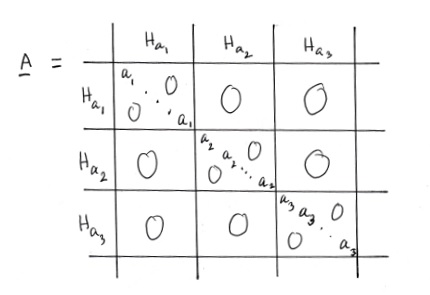
\includegraphics[scale=0.90]{A.jpg}
\vspace{-0.8 cm}
\caption{The matrix representation of $\hat{A}$ in the eigenbasis of $\hat{A}$. }
\label{afig:A}
\end{figure}

\noindent
where each diagonal block $H_{a_n}$ is a $g_{a_n}\times g_{a_n}$ dimensional diagonal matrix with the eigenvalue $a_n$ running
along the diagonal, other entries being zero.


\paragraph{}
Next, we ask what would be the matrix representation of $\hat{B}$ in the eigenbasis of $\hat{A}$. The matrix elements
of $\hat{B}$ are written as 
$\langle a^{\prime}, i^{\prime}|\hat{B}|a,i\rangle$. Using our assumption that $\hat{A}$ and $\hat{B}$ commute, we have
\be
\langle a^{\prime}, i^{\prime}|[\hat{A},\hat{B}]|a,i\rangle = 0,\nonumber
\ee
i.e.,
\be
\langle a^{\prime}, i^{\prime}|\hat{A}\hat{B}-\hat{B}\hat{A}|a,i\rangle = 0, \nonumber
\ee
or,
\be
(a^{\prime}-a)\langle a^{\prime}, i^{\prime}|\hat{B}|a,i\rangle=0.
\ee
If $a\neq a^{\prime}$, then $(a^{\prime}-a)\neq 0$ and we must have
\be
\langle a^{\prime}, i^{\prime}|\hat{B}|a,i\rangle =0, \quad {\rm if} \; a^{\prime}\neq a,
\label{aeq:matrixelement}
\ee
i.e., $\hat{B}$ does not connect states with different eigenvalues of $\hat{A}$. In other words, $\hat{B}$ acting
on any of the eigenvectors of $\hat{A}$ in the eigensubspace $H_a$, produces another vector which is also in $H_a$ with no components in other eigensubspaces orthogonal to $H_a$. The new vector, being in $H_a$, remains an eigenvector of $\hat{A}$. Thus, $\hat{B}$
acting on any eigenvector of $\hat{A}$ produces a state which is also an eigenvector of $\hat{A}$ with the same eigenvalue. This is a
consequence of the fact that $\hat{A}$ and $\hat{B}$ commute.

\paragraph{}
From the above arguments, we can conclude that the matrix representation of $\hat{B}$ in the eigenbasis of $\hat{A}$
will be block diagonal as shown below.
\begin{figure}[ht]
\centering
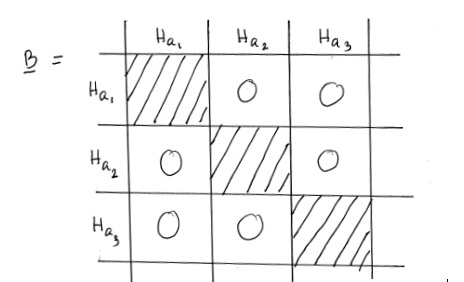
\includegraphics[scale=1.0]{B.jpg}
\vspace{-3 mm}
\caption{The matrix representation of $\hat{B}$ in the eigenbasis of $\hat{A}$. }
\label{afig:B}
\end{figure}

\noindent
In each eigensubspace $H_a$, the matrix ${\underline B}^{(a)}$ is a $g_a \times g_a$ square matrix, which itself need not be diagonal if we choose an arbitrary basis for $H_a$. To see this we refer to Eq. (\ref{aeq:matrixelement}). This equation tells us that, 
if $\hat{A}$ and $\hat{B}$ commute, the matrix elements of $B$ are zero if $a\neq a^{\prime}$, but nothing is concluded about
the matrix elements of $\hat{B}$ in any eigensubspace $H_a$, i.e., when $a=a^{\prime}$. 

\paragraph{}
However, since $\hat{B}$ is a Hermitian operator, its matrix representation in every eigensubspace $H_a$, is a finite dimensional square Hermitian matrix. We can always diagonalize a finite dimensional Hermitian matrix by a change of basis. The new set of $g_a$ basis vectors in the eigensubspace $H_a$ are linear combinations of the old basis vectors 
$\{ |a,i\rangle, i=1,2, \cdots , g_a\}$. Therefore, the vectors of the new basis set remain eigenvectors of $\hat{A}$ with the same eigenvalue $a$. But, the vectors in  new basis set, since it diagonalizes $\hat{B}$, must also 
be eignevectors of $\hat{B}$ with eigenvalues $b_1,b_2,b_3, \cdots$ where some of the $b_i's$ may be repeated.

\paragraph{}
Since the vectors in the new basis set are simultaneous eigenvectors of $\hat{A}$ and $\hat{B}$, we can label them by the eigenvalues of both $\hat{A}$ and $\hat{B}$. Thus the common eigenvectors, which form the new basis set of $H_a$, can be written as
$\{ |a,b_1\rangle, |a,b_2\rangle, \cdots , |a, b_{g_a}\rangle \}$ provided the $b_i's$ are distinct. Some of the eigenvalues of $\hat{B}$ may be repeated, in which 
case we will need another index to distinguish between the linearly independent simultaneous eigenvectors with the same 
values for the eigenvalue pair $(ab_i)$. We diagonalize each diagonal block $\underline{B}^{(a_i)}$ of the matrix 
$\underline{B}$ in the old basis, thereby obtaining simultaneous eigenvectors for both $\hat{A}$ and $\hat{B}$ in each eigensubspace.
The set of simultaneous eigenvectors in all eigensubspaces $H_a, a\in {\rm spec}(\hat{A})$ can now be used as the basis set for
the Hilbert space. In the new basis consisting of the simultaneous eigenvectors,  the matrix representation of $\hat{B}$ is diagonal as shown in  figure (\ref{afig:C}). The matrix representation of $\hat{A}$ in the new basis is also diagonal and remains the same as in Fig. (\ref{afig:A}). 


\begin{figure}[ht]
\centering
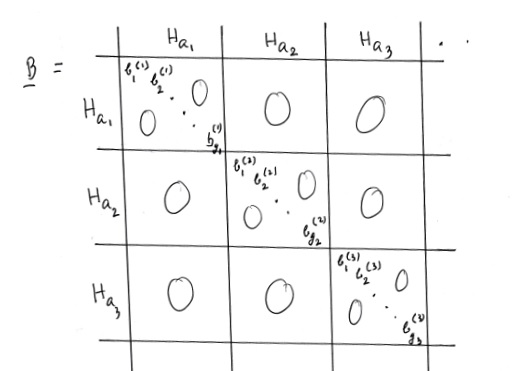
\includegraphics[scale=1.0]{C.jpg}
\vspace{-6 mm}
\caption{The matrix representation of $\hat{B}$ in the eigenbasis consisting of simultaneous eigenvectors of
$\hat{A}$ and $\hat{B}$.}
\label{afig:C}
\end{figure}



\paragraph{}
The diagonal entries $b_i^{(n)}, i=1,2, \cdots , g_n$ in each eigensubspace $H_{a_n}$ in figure (\ref{afig:C}) are the various eigenvalues of the operator $\hat{B}$, i.e., $b_i^{(n)} \in \{b_1,b_2, \cdots\}$. In a given eigensubspace $H_{a_n}$, some of the eigenvalues of
$\hat{B}$ may be repeated. Further, a particular eigenvalue of $\hat{B}$ may also be repeated in several eigensubspaces $H_{a_n}$.

\paragraph{}
Thus, in summary, what we have shown is that, given two Hermitian operators $\hat{A}$ and $\hat{B}$ representing
two observables of a quantum system,  it is possible to construct a complete set of simultaneous eigenvectors 
spanning the entire Hilbert space provided  $[\hat{A},\hat{B}]=0$. Hence, we have proved that $[\hat{A},\hat{B}]=0$ is a sufficient condition for two Hermitian operators $\hat{A}$ and $\hat{B}$ to be compatible.


% New section
% Sec 5
\section{Labeling of Quantum Mechanical Basis States}
Since eigenvectors of a Hermitian operator corresponding to an observable form a complete set, we can label the members of the set by the eigenvalues. Thus, suppose that an observable $\hat{A}$ has eigenvalues
\[ a_1, a_2, a_3, \cdots\, . \]
The basis states are then labeled as
\[ |a_1\rangle,\, |a_2\rangle,\, |a_3\rangle,\, \cdots \, . \]
The labeling would be unambiguous if the eigenvalues were all non-degenerate. However, if some or all eigenvalues are degenerate, we will need another mark of distinction for the eigenvectors. 

\paragraph{}
For example, if an eigenvalue $a_n$ is $g_n$-fold degenerate, the corresponding eigenvectors may be denoted as
\[ |a_n,i\rangle,\, i=1,2, \cdots , g_n\, . \]
An alternative, and better, notation is based on the fact that two compatible observables whose Hermitian operators commute, may be assumed to have the same set of eigenvectors. Hence, if we can find a second observable $\hat{B}$ commuting with the first, such that
\be
\hat{B}|a_n,i\rangle = b_i|a_n,i\rangle,\, i=1,2, \cdots , g_n 
\ee
with eigenvalues $b_i$ all different, then the eigenvalues of $\hat{B}$ may serve to distinguish the eigenvectors.
So, we can write
\[
\begin{array}{lcl}
|a_n,1\rangle & \equiv & |a_n,b_1\rangle \\
|a_n,2\rangle & \equiv & |a_n,b_2\rangle \\
. & & . \\
. & & . \\
. & & . \\
|a_n,g_n\rangle & \equiv & |a_n,b_{g_n}\rangle\, . 
\end{array}
\]
But, if some of the eigenvalues $b_i, i=1,2, \cdots, g_n$ are equal, we will need a third mark to distinguish the eigenvectors. The third mark may be obtained if we can find a third observable whose operator $\hat{C}$ commutes with both $\hat{A}$ and 
$\hat{B}$. Then $\hat{A}$, $\hat{B}$ and $\hat{C}$ have simultaneous eigenvectors and the eigenvalues of $\hat{C}$ may also be used to label the eigenvectors.

\paragraph{}
Thus, in general, if we can find a set of mutually commuting Hermitian operators, $\hat{A},\hat{B},\hat{C},\hat{D} , \cdots $
whose common eigenvectors can be characterized completely by the eigenvalues $a,b,c,d, \cdots$ such that no two eigenvectors have exactly identical set of eigenvalues, then the eigenvalues of these operators can uniquely label the common eigenvectors.
Such a set of Hermitian operators is said to be complete. We refer to this set of operators as a complete set of commuting 
observables (CSCO). 

\paragraph{}
In the new notation, the basis vectors are written as
\[ |a,b,c, d, \, \cdots \rangle \, . \]
The normalization and completeness conditions are then 
\be
\langle a^{\prime},b^{\prime},c^{\prime}, d^{\prime} \cdots |a,b,c,d,\cdots \rangle = \delta_{aa'}\delta_{bb'} \cdots \, ,
\ee
and
\be
\sum_{(a,b,c,d,\cdots)} |a,b,c,d,\cdots \rangle \langle a,b,c,d,\cdots |= \hat{I} \, . 
\ee









